\section{Experimental Results}\label{sec:results}

In this section we discuss our experimental evaluation of the work profiling strategies and 
the effectiveness of the work efficiency metric on guiding true online {\itercomp}.
We use the following naming convention for the profiling strategies considered
throughout this section:
\begin{itemize}[leftmargin=3mm]
\item \textbf{\OracleRM} measures the actual speedup over the unoptimized version of the program for any given input.
In our experiments, this oracle is allowed to execute each input at least twice so the speedup can be computed.
\item \textbf{\OraclePP} measures the work efficiency metric with a \textit{magically perfect} non-intrusive profiling.
  Because this version simulates a \textit{perfect} profiling, with zero overhead,
  it allows us to isolate and evaluate the actual effectiveness of the work efficiency metric.
\item \textbf{\OptProf} corresponds to the work profiling using the optimal placement of the probes.
  This profiling strategy requires a single execution of the program for any given input.
\item \textbf{\WCRelax-\textit{N}\%} measures the work efficiency metric using the work profiling with a \textit{N}\% threshold for
the \WCRelaxLower relaxation.
  Similar to the \OptProf, this profiling strategy also requires a single execution of the program for any given input.
\item \textbf{\WPRelax-\textit{N}\%} is similar to the \WCRelax, but it applies the \WPRelaxLower relaxation instead.
\end{itemize}

\begin{figure*}[t!]
    \centering
    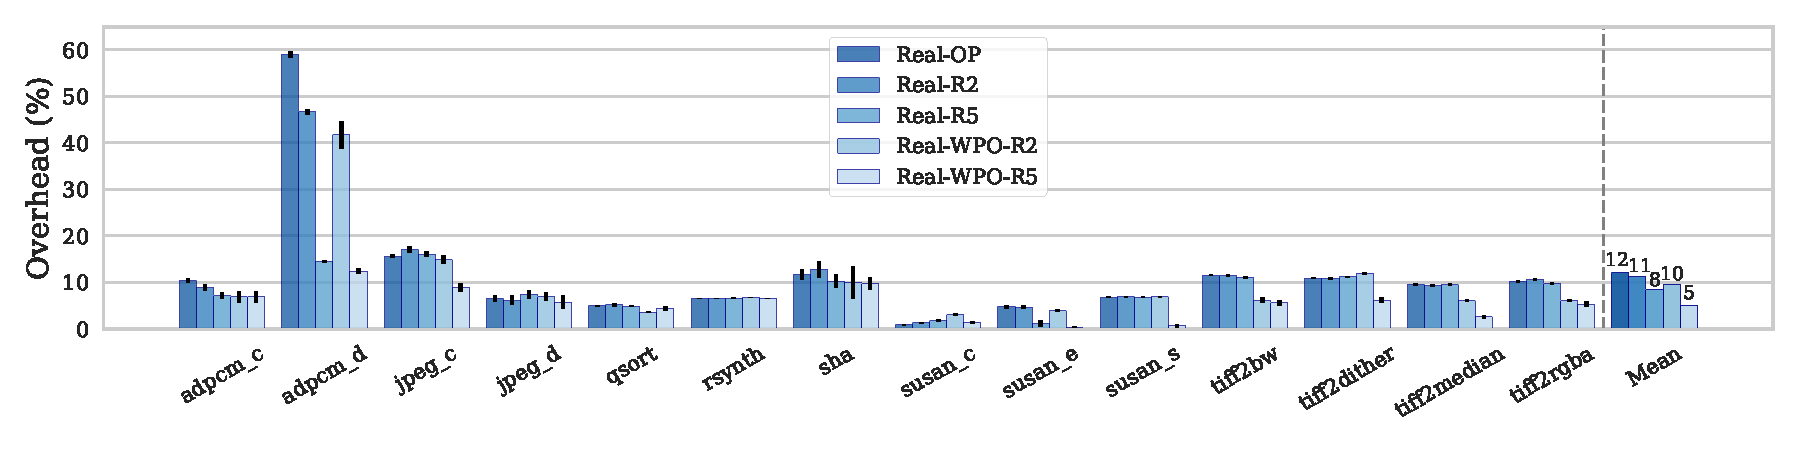
\includegraphics[width=\textwidth]{figs/overhead-O3.pdf}
    \caption{Instrumentation overhead for each benchmark averaged over all inputs, when compiled with {\flagstype -O3}.}
    \vspace{-3mm}
    \label{fig:overhead-O3}
\end{figure*}

\begin{figure*}[t!]
    \centering
    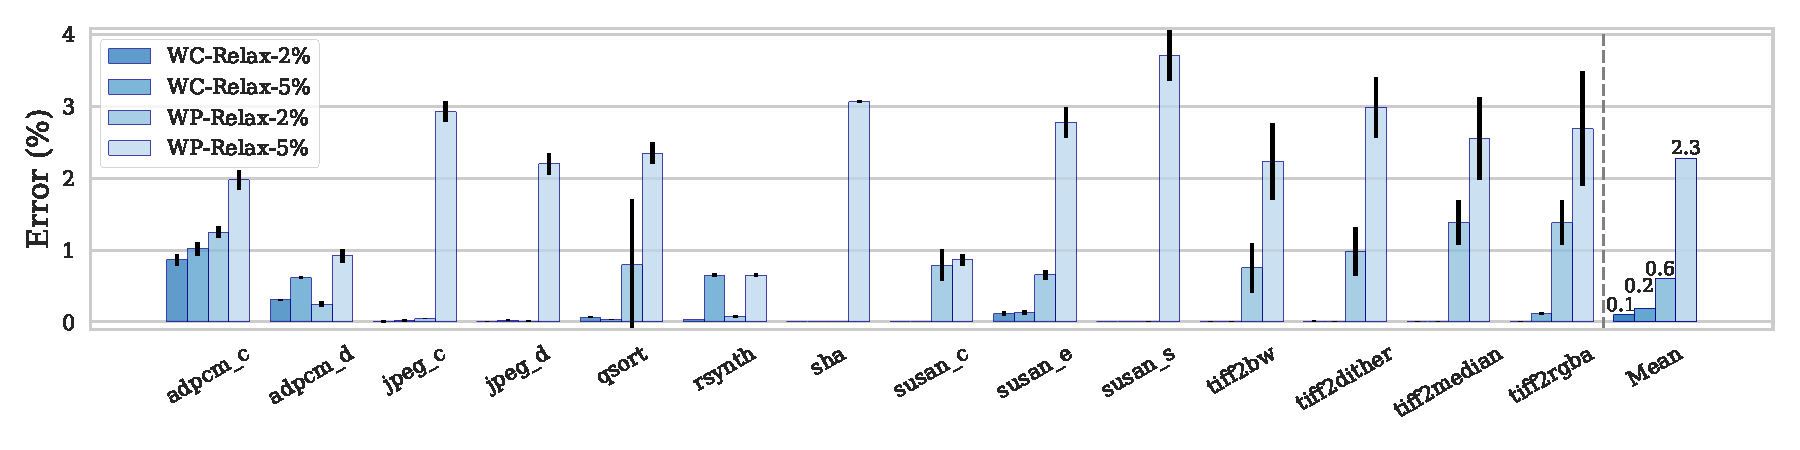
\includegraphics[width=\textwidth]{figs/error-O3.pdf}
    \caption{Dynamic error of the work profiling averaged over the 1000 inputs, after relaxing the number of probes.}
    \vspace{-3mm}
    \label{fig:error-O3}
\end{figure*}

%Mean values...
%Real-R5: 30.43\%
%WPO-R5:  54.97\%
%adpcm_d:
%Real-R5: 75.51\%
%WPO-R5:  79.07\%

\subsection{Evaluation of the Instrumentation}

First, we evaluate the runtime overhead introduced by the work efficiency profiling. A high overhead would impact the user's experience
and would make our approach impractical. We take the original and instrumented versions of each benchmark, we compile them using the
baseline \texttt{-O3} setting, and execute them with all 1,000 inputs. The difference in their runtimes, for the same input, is the
instrumentation overhead. Figure~\ref{fig:overhead-O3} shows the average overhead for each benchmark and work profiling strategy. 

\OptProf typically slows the application down by 10\%, noticeably affecting the user experience, while in the worst case its overhead
reaches 59\%. It is clearly unsuitable for online work profiling. \WCRelax and \WPRelax fare better, especially when used with a higher
5\% threshold. \WPRelax-\textit{5}\%, in particular, has an average overhead of only 5\%, 13\% in its worst case. 

For almost all the profiling strategies, their worst case is \texttt{adpcm\_d}. Still, compared to the 59\% overhead of the \OptProf,
\WCRelax-\textit{5}\% and \WPRelax-\textit{5}\% incur only about a quarter of that overhead. This benchmark has a single hot function
consisting mainly of a single hot loop with several branches inside it. Most of the overhead comes from two probes which are placed in
very frequently executed blocks but contribute little to the total work of the loop. The maximum possible error caused by removing either
of the probes, based on the analysis of the DAG, is about 1.3\%. Both relaxation strategies identify this opportunity and remove the probes.

Some benchmarks display unexpectedly higher overheads under the relaxation strategies. This is counter-intuitive because relaxation only
reduces the number of instrumented probes without changing their placement. By analyzing these cases, we noticed that we could not remove
the most frequently executed probes, so relaxation had little positive impact. At the same time, we removed some probes which were
infrequently executed but were taken into consideration by the LLVM optimization heuristics. In some cases, removed probes caused different
and suboptimal decisions to be made, increasing the runtime. 

Figure~\ref{fig:error-O3} shows that profiling with relaxation incurs very little dynamic error. It also confirms that the \WCRelaxLower
relaxation is overly conservative, while the \WPRelaxLower relaxation achieves a better trade-off. Although the error bound is not
guaranteed by the \WPRelaxLower relaxation, its dynamic error is always below the 5\% threshold. For both relaxation strategies the 2\%
threshold is too conservative to be useful. The rest of the paper only evaluates the 5\% threshold.

\subsection{Evaluation of Online {\IterComp}}

\begin{figure*}[t]
    \centering
    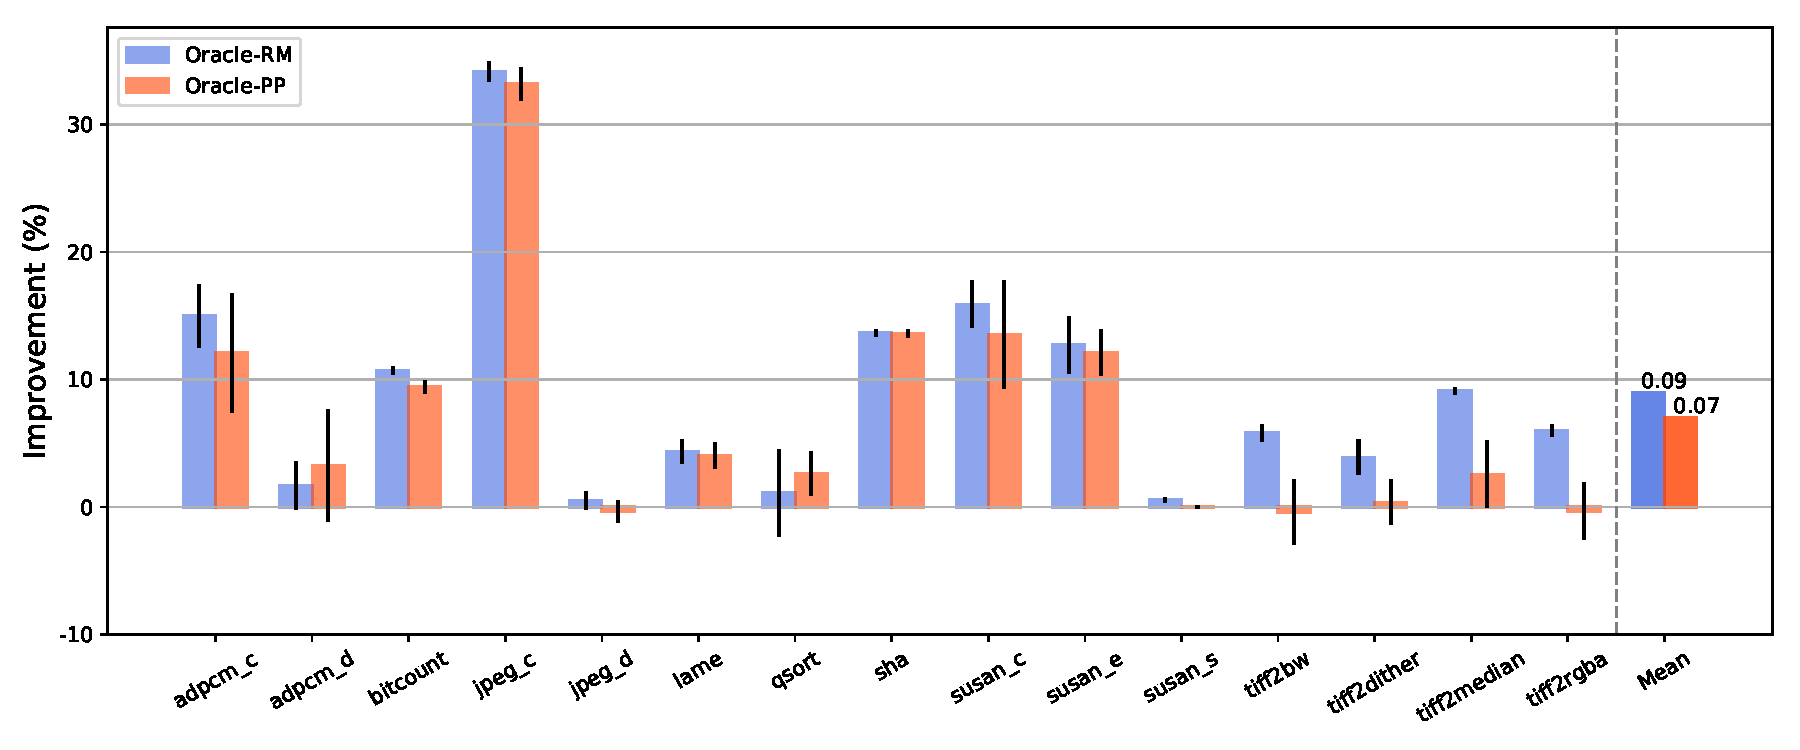
\includegraphics[width=\textwidth]{figs/speedups.pdf}
    \caption{Speedups obtained from the final optimization sequence selected by the online {\itercomp}.
	         The speedups reported for each benchmark represents the average speedup across their complete 1000 input datasets.}

    \FIXME{Sort  the bars according to speedup, i.e. Oracle should be the last bars.}
    \label{fig:speedups}
\end{figure*}

In this section we evaluate the effectiveness of our work efficiency metric.
We perform online {\itercomp} using all five profiling strategies, namely
\OracleRM, \OraclePP,\OptProf,\WCRelax-5\%, and \WPRelax-5\%.
Because the \OracleRM measures actual speedup, it provides reference results for
assessing the effectiveness of the work-efficiency metric.

For all strategies, the same optimization sequence is used for multiple inputs, using a dynamic input-window size, as explained in
Section~\ref{sec:oic-infra}. The average performance over the input window provides an estimate for the overall performance of the
optimization sequence across distinct inputs. The optimization sequences are ranked based on their average performance, and the best
optimization sequence is selected.

The comparison between \OracleRM and \OraclePP is crucial for validating the
effectiveness of the work efficiency metric in guiding online {\itercomp},
while the other configurations demonstrate the viability of applying online
{\itercomp} in real-world scenarios.

In order to evaluate the quality of the final optimization sequences selected by each configuration of the online {\itercomp}, we compare
their speedup over the \texttt{-O3} optimization across all the 1,000 inputs of the benchmark being optimized. None of the configurations
degrades the performance over \texttt{-O3} (with statistical significance).
%When measuring the wall-clock time for each input, to reduce noise, we execute
%the same input until we have a statistically sound measurement, i.e. we execute
%until we have an interval no larger than 1\% with 99\% confidence.
Figure~\ref{fig:speedups} shows these average speedups for all test benchmarks.
This figure shows that the best optimization sequence selected with the Oracle-PP
is very close to the performance of the best optimization sequence selected with
the \OracleRM, where \OraclePP achieves on average about 80\% of the performance
improvement obtained by the \OracleRM.
This result is important for demonstrating that our work efficiency metric has
the potential to produce good results in real-world online scenarios.

The \OptProf achieves 4\% improvement on average, which represents 45\% of the
performance improvement obtained by the \OracleRM.
This difference to \OraclePP is explained by the real (intrusive) profiling used
in the \OptProf configuration.
The profiling affects the search in two key ways:
\textit{(i.)} the overhead incurred by the profiling affects the execution time,
and therefore also affects the work efficiency metric,
\textit{(ii.)} the instrumentation code may affect many of the optimizations, e.g.,
due to the use of a global variable or in decisions taken based on a cost-model
for the instructions.
However, even in the \OptProf configuration, which has a highly intrusive instrumentation,
it is still possible to obtain performance improvements in a realistic online
{\itercomp}.

Finally, the evaluation also indicates that the use of relaxation algorithms
is beneficial not only for its reduction in overhead, which is directly observed
by the user, by it also tends to improve the quality of the search.
This improvement has to do with the aforementioned effects of an intrusive
instrumentation on the search.
The relaxation has the potential to reduce both effects of the profiling.
Both the \WCRelax-5\% and \WPRelax-5\% achieve about 60\% of the
performance improvement obtained by the \OracleRM.
